\documentclass[11pt,a4paper]{article}

% ============================================================================
% PACKAGES
% ============================================================================
\usepackage[utf8]{inputenc}
\usepackage[french]{babel}
\usepackage[T1]{fontenc}
\usepackage{graphicx}
\usepackage{float}
\usepackage{amsmath}
\usepackage{amssymb}
\usepackage{geometry}
\usepackage{fancyhdr}
\usepackage{hyperref}
\usepackage{listings}
\usepackage{xcolor}
\usepackage{subcaption}
\usepackage{enumitem}
\usepackage{tikz}
\usetikzlibrary{shapes.geometric,arrows}

\graphicspath{{/Users/nathan/Documents/Scolarite/ISIMA/ZZ3/blender/geom-algo-segmentation TP4/output/renders}}
% ============================================================================
% MISE EN PAGE
% ============================================================================
\geometry{
    left=2.5cm,
    right=2.5cm,
    top=2.5cm,
    bottom=2.5cm
}

\pagestyle{fancy}
\fancyhf{}
\rhead{TP3 - Segmentation de maillage}
\lhead{ISIMA ZZ3}
\rfoot{\thepage}

% ============================================================================
% COULEURS POUR CODE
% ============================================================================
\definecolor{codegreen}{rgb}{0,0.6,0}
\definecolor{codegray}{rgb}{0.5,0.5,0.5}
\definecolor{codepurple}{rgb}{0.58,0,0.82}
\definecolor{backcolour}{rgb}{0.95,0.95,0.92}

\lstdefinestyle{mystyle}{
    backgroundcolor=\color{backcolour},   
    commentstyle=\color{codegreen},
    keywordstyle=\color{magenta},
    numberstyle=\tiny\color{codegray},
    stringstyle=\color{codepurple},
    basicstyle=\ttfamily\footnotesize,
    breakatwhitespace=false,         
    breaklines=true,                 
    captionpos=b,                    
    keepspaces=true,                 
    numbers=left,                    
    numbersep=5pt,                  
    showspaces=false,                
    showstringspaces=false,
    showtabs=false,                  
    tabsize=2
}
\lstset{style=mystyle}

% ============================================================================
% HYPERLINKS
% ============================================================================
\hypersetup{
    colorlinks=true,
    linkcolor=blue,
    filecolor=magenta,      
    urlcolor=cyan,
    citecolor=blue
}

% ============================================================================
% TITRE
% ============================================================================
\title{
    \vspace{-2cm}
    \textbf{TP4 : Lissage et déformation}\\
    \large Géométrie Algorithmique - ISIMA F1
}

\author{
    \textbf{Nathan BERT}\\
    \small ISIMA - ZZ3\\
    \small \texttt{nathan.bert@etu.uca.fr}
}

\date{25 mars 2026}

% ============================================================================
% DOCUMENT
% ============================================================================
\begin{document}

\maketitle
\vspace{4cm}

\begin{abstract}
Ce rapport présente le travail réalisé dans le cadre du TP4 de la matière géométrie algorithmique portant 
sur le lissage de maillages 3D. L'objectif du TP est d'implémenter et de comparer différentes méthodes de lissage,
afin de mieux appréhender l'impact de modifications locales d'un maillage portées à une échelle globale.
Le parcours et la modification des maillages se feront à l'aide de la librairie CGAL.\\
Nous aborderons dans un premier temps les approches de lissage les plus simples, à savoir le lissage laplacien uniforme
et son extension par facteur de diffusion, avant de présenter la méthode de Taubin qui corrige le phénomène
de rétrécissement inhérent aux approches précédentes. Nous verrons ensuite les différentes stratégies de pondération
du lissage laplacien. L'ensemble de ces méthodes sera enfin confronté 
visuellement et discuté à travers une série de rendus en fil de fer générés automatiquement sur un maillage bruité commun, (à noter que tous les rendus visuels des maillages se trouvent dans le dossier /output/renders à partir de la racine du projet C++).\\
Par souci de transparence quant à mon usage des outils de génération automatique, je tiens à préciser que le code
produit a entièrement été commenté à l'aide de l'intelligence artificielle, en se basant sur \href{https://ntrs.nasa.gov/citations/20080039927}{le guide de style de la NASA},
et que je m'en suis également servi pour créer la fonction de visualisation des maillages. 
Le reste du code et la logique implémentée sont cependant ma production.
\end{abstract}
\newpage

\tableofcontents
\newpage
\listoffigures

\newpage

\section{Contexte}

Souvent lorsque l'on manipule des maillages de points 3D, ceux-ci représentent un objet du réel
ou sont issus de relevés mêmes de points sur ce même objet pour en obtenir une représentation virtuelle.
Les points extraits peuvent néanmoins présenter des irrégularités, provenant de bruits de mesures ou encore se 
retrouver discrétisés en voxels pour une représentation moins couteuse en mémoire.\\
Afin de pouvoir exploiter ces maillages, il nous faut alors pouvoir gommer ces imperfections et artefacts.
Une des solutions à notre disposition est d'appliquer un algorithme de lissage sur le maillage afin normaliser les erreurs locales.\\
Dans notre cas et dans ce TP nous manipulerons des maillages sur lesquels ont été appliqués différents bruits d'intensités différentes et 
nous observerons l'impact que peuvent avoir différents types de lissages existants sur ces maillages.

\newpage

\section{Le Lissage Simple}
Lorsque l'on parle de lissage, l'une des premières solutions que l'on pourrait être tenté d'aborder serai d'uniformiser de manière individuelle chaque point par rapport à ses voisins directs.
Une des façons de faire cela est pour chaque point prendre les coordonnées sur chaque axe de ses voisins et de calculer le centroïde (\textit{centre de masse}) de cette structure. 
On place notre point dans le nouveau maillage aux coordonnées de ce centroïde sans changer sa position dans le maillage initial pour ne pas altérer les futurs calculs de centroïdes l'impliquant, 
puis l'on recommence pour chaque point du maillage.


\subsection{Exemple : point intérieur d'un triangle}

Triangle $ABC$ : $A(0,0)$, $B(4,0)$, $C(2,3)$. Points intérieurs $P(1.5,1)$ et $K(3,0.7)$ (voisins : $A,B,C$).\\

Centroïde : $\mathbf{c}_P = \frac{A + B + C}{3} = \left( \frac{6}{3}, \frac{3}{3} \right) = (2,1)$.\\

Déplacement : $\Delta_P = (0.5, 0)$ vers $P' = (2,1)$ et  $\Delta_K = (-1, 0.3)$ vers $K' = (2,1)$

\begin{center}
\begin{tikzpicture}[scale=1.8, every node/.style={font=\small}]
    % Triangle
    \draw[thick,blue] (0,0) -- (4,0) -- (2,3) -- cycle;
    \fill[blue!20] (0,0) circle (2pt) node[below left] {$A$};
    \fill[blue!20] (4,0) circle (2pt) node[below right] {$B$};
    \fill[blue!20] (2,3) circle (2pt) node[above] {$C$};
    
    % Point P initial
    \fill[orange!70!black] (1.5,1) circle (3pt) node[below left] {$P$};
    \fill[black!70!black] (3,0.7) circle (3pt) node[below left] {$K$};
    
    % Centroïde
    \fill[red] (2,1) circle (3pt) node[above right] {$\mathbf{c}_P$};
    
    % Flèche déplacement
    \draw[red,->,thick] (1.5,1) -- (2,1) node[midway,above] {$\Delta_P$};
    \draw[blue,->,thick] (3,0.7) -- (2,1) node[midway,above] {$\Delta_K$};
    
    % P après
    \fill[green!70!black] (2,1) circle (3pt) node[below left] {$P'$};
    \fill[blue!70!black] (2,1) circle (2pt) node[below right] {$K'$};
    
    % Lignes aux centroïdes pour visualisation
    \draw[dashed,gray] (2,1) -- (0,0);
    \draw[dashed,gray] (2,1) -- (4,0);
    \draw[dashed,gray] (2,1) -- (2,3);
\end{tikzpicture}
\end{center}

Les points $P$ et $K$ migrent vers le centroïde du triangle (moyenne des 3 voisins).


% \begin{center}
% 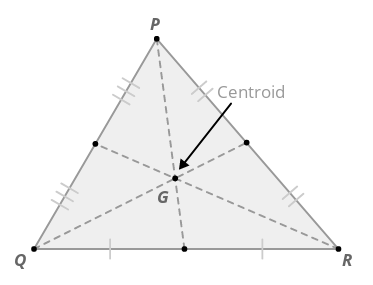
\includegraphics[scale=0.5]{./images/IG_4_6_0_a_Centroid.png}
% \captionof{figure}{Illustration du centroïde sur un triangle}
% \label{figure_centroide}
% \end{center}

\subsection{Facteur de Diffusion}
Dans l'approche précédemment expliquée, nous remarquons que la nouvelle position du point est calculée de manière indépendante à sa position intiale vis à vis de ses voisins.
Peu importe la position initale du point, celui-ci se retrouvera à la même position relative pour un même voisinage.
Cette approche aura donc tendance à uniformiser les aires des surfaces dans le maillage. Cela peut avoir pour conséquence la disparition de détails locaux mais également à un regroupement généralisé des points dont nous rediscuterons dans une partie ultérieure.
afin de conserver une partie de l'information du point, nous pouvons pondérer le vecteur déplacement obtenu pour déplacer le point quelque part entre
sa position initiale et le centroïde. \\

Formellement, la nouvelle position devient :
\begin{equation}
\mathbf{p}_v' = \mathbf{p}_v + \alpha \cdot \Delta_v = (1 - \alpha) \mathbf{p}_v + \alpha \cdot \mathbf{c}_v,
\end{equation}
où $\alpha \in [0,1]$ est le \textbf{facteur de diffusion}. Pour $\alpha=1$, on retrouve le lissage simple ; pour $\alpha<1$, le lissage est progressif et préserve mieux la géométrie globale.

\newpage
\newpage

\section{Lissage de Taubin}
L'application répétée d'un lissage laplacien uniforme ou avec facteur de diffusion pose un problème géométrique majeur : le phénomène de rétrécissement (\textit{shrinkage}). En effet, en déplaçant itérativement les sommets vers le centroïde de leurs voisins, le volume global du maillage diminue inévitablement, conduisant à terme à l'effondrement de la structure sur elle-même.

Pour pallier ce problème, la méthode de Taubin propose une approche en deux temps, s'apparentant à un filtre passe-bas pour la géométrie. À chaque itération, l'algorithme alterne deux phases :
\begin{enumerate}
    \item \textbf{Une phase de contraction (\textit{shrink})} : on applique un déplacement laplacien avec un facteur de diffusion positif $\lambda > 0$.
    \item \textbf{Une phase de dilatation (\textit{inflate})} : on applique un déplacement avec un facteur négatif $\mu < 0$, afin de repousser les sommets vers l'extérieur et compenser la perte de volume.
\end{enumerate}

Pour garantir la stabilité et une convergence efficace, il est impératif que $|\mu| > \lambda$. En se reposant sur les valeurs proposées par le sujet du TP, des valeurs telles que $\lambda = 0.33$ et $\mu = -0.34$ offrent des résultats intéressant. Le maillage est ainsi lissé des bruits hautes fréquences tout en conservant son volume initial.

\newpage

\section{Lissage Laplacien Pondéré}

\subsection{Notion de Facteur}
Le calcul du centroïde de manière équiprobable considère que chaque sommet voisin a une influence identique sur la nouvelle position. Cependant, dans des maillages hétérogènes où la densité des points ou la forme des triangles varie fortement, cette approche déforme la topologie locale.
L'idée du lissage pondéré est d'introduire un poids $w_{ij}$ pour chaque arête reliant le sommet $i$ à son voisin $j$. La nouvelle position devient alors une somme pondérée :
\begin{equation}
\mathbf{p}_i' = \frac{\sum_{j \in N(i)} w_{ij} \mathbf{p}_j}{\sum_{j \in N(i)} w_{ij}}
\end{equation}

\subsubsection{Facteur Uniforme}
Il s'agit du cas où $w_{ij} = 1$ pour tout voisin $j$. On retrouve alors exactement l'équation du lissage laplacien simple détaillé précédemment, qui calcule le barycentre géométrique du voisinage sans tenir compte des distances ou des courbures.
\subsubsection{Facteur Inverse}
Une première amélioration consiste à pondérer l'influence d'un voisin par l'inverse de la distance qui le sépare du sommet courant :
\begin{equation}
w_{ij} = \frac{1}{\| \mathbf{p}_i - \mathbf{p}_j \|}
\end{equation}
Ainsi, un sommet géométriquement proche aura un impact plus fort sur le déplacement qu'un sommet éloigné. Bien que simple à implémenter, cette méthode reste sensible aux irrégularités de maillage et ne reflète pas parfaitement la courbure de la surface.

\subsubsection{Facteur basé sur les Cotangentes}
Afin d'obtenir un lissage qui respecte véritablement la géométrie de la surface, on utilise les poids cotangents. Pour une arête reliant $i$ et $j$, partagée par deux triangles dont les angles opposés à l'arête sont $\alpha_{ij}$ et $\beta_{ij}$, le poids est donné par :
\begin{equation}
w_{ij} = 0.5 \times (\cot \alpha_{ij} + \cot \beta_{ij})
\end{equation}
L'implémentation robuste de ce facteur implique l'utilisation du produit scalaire et du produit vectoriel des arêtes adjacentes. Cette méthode prend en compte l'aire et les angles des faces, ce qui permet de lisser le bruit tout en préservant très fidèlement les arêtes vives et la forme globale du modèle originel.

\newpage

\section{Résultats et Discussions}

Afin de comparer rigoureusement les différentes approches de lissage implémentées, nous avons appliqué nos algorithmes sur un maillage de référence présentant un bruit artificiel (\texttt{cube-bruit.off}). Cette démarche nous permet d'observer l'impact de chaque méthode sur une topologie identique et d'évaluer leur capacité à filtrer les hautes fréquences tout en préservant les caractéristiques géométriques globales du modèle.

\subsection{Comparaison visuelle des méthodes}

\subsubsection{Le Mesh Cube}


La figure \ref{fig:comparaison_lissages} présente l'évolution du maillage d'un cube initialement bruité avant et après l'application de nos différents lissages. 
Grâce à notre script d'automatisation de rendu en fil de fer, nous pouvons distinctement observer la structure topologique et la répartition des sommets.

\begin{figure}[H]
    \centering
    \begin{subfigure}[b]{0.32\textwidth}
        \centering
        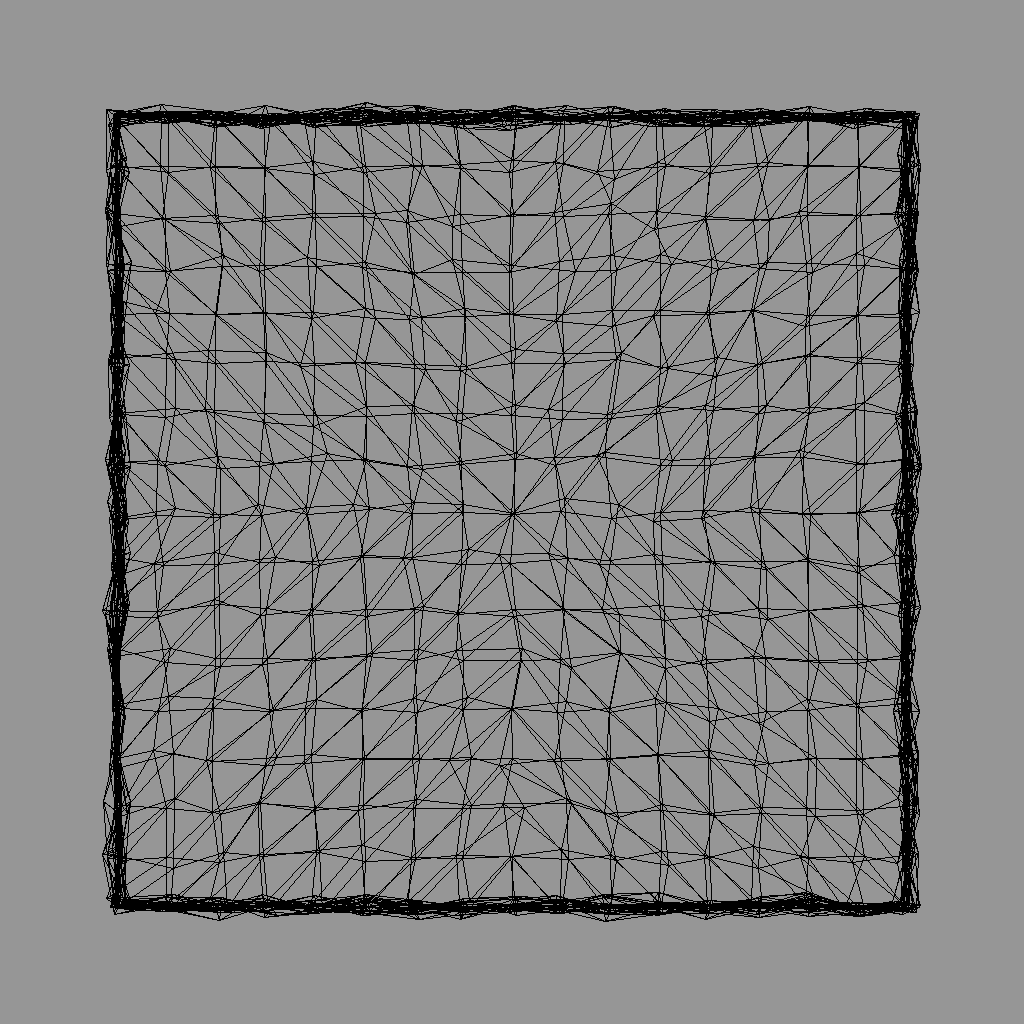
\includegraphics[width=\textwidth]{../output/renders/cube-bruit-0.png} 
        \caption{Maillage original bruité}
        \label{fig:res_original}
    \end{subfigure}
    \hfill
    \begin{subfigure}[b]{0.32\textwidth}
        \centering
        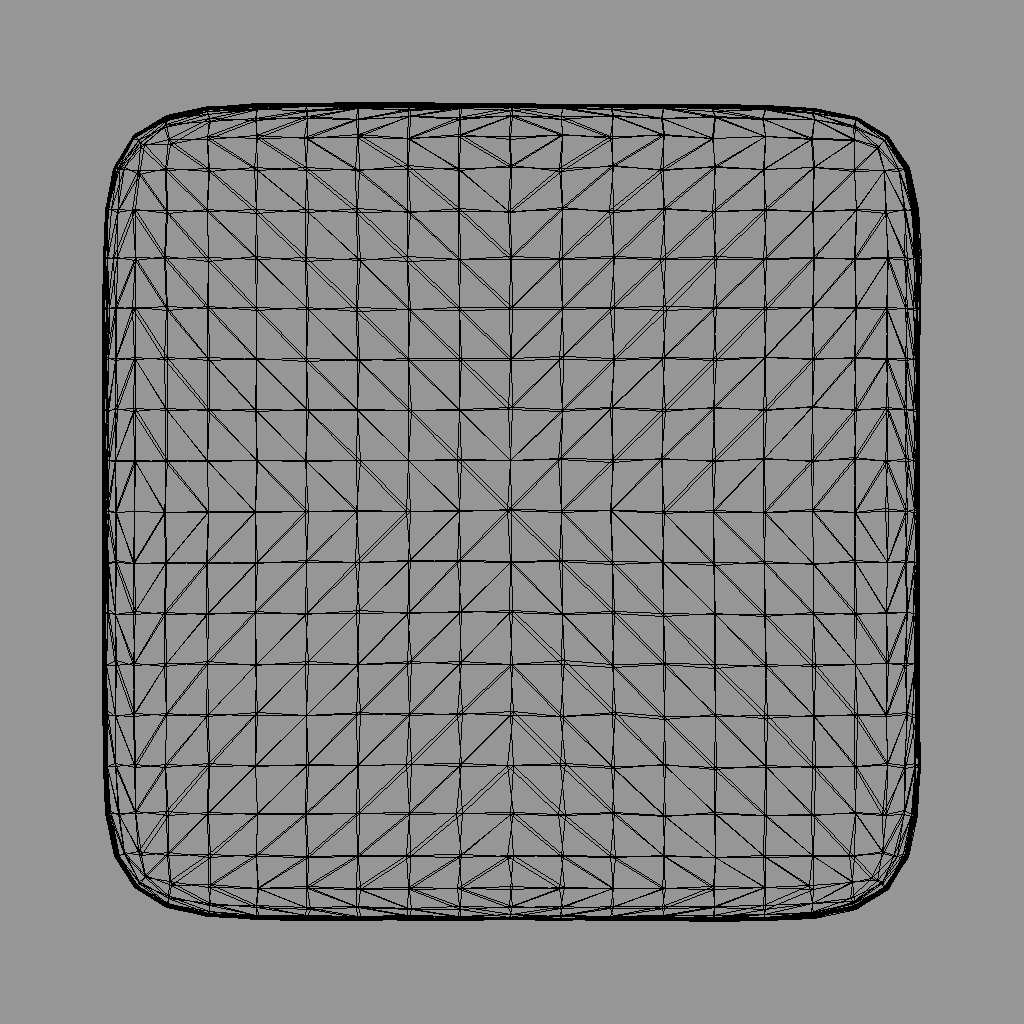
\includegraphics[width=\textwidth]{../output/renders/cube-bruit-0_LissageLaplacien_5.png}
        \caption{Laplacien Uniforme}
        \label{fig:res_laplacien}
    \end{subfigure}
    \hfill
    \begin{subfigure}[b]{0.32\textwidth}
        \centering
        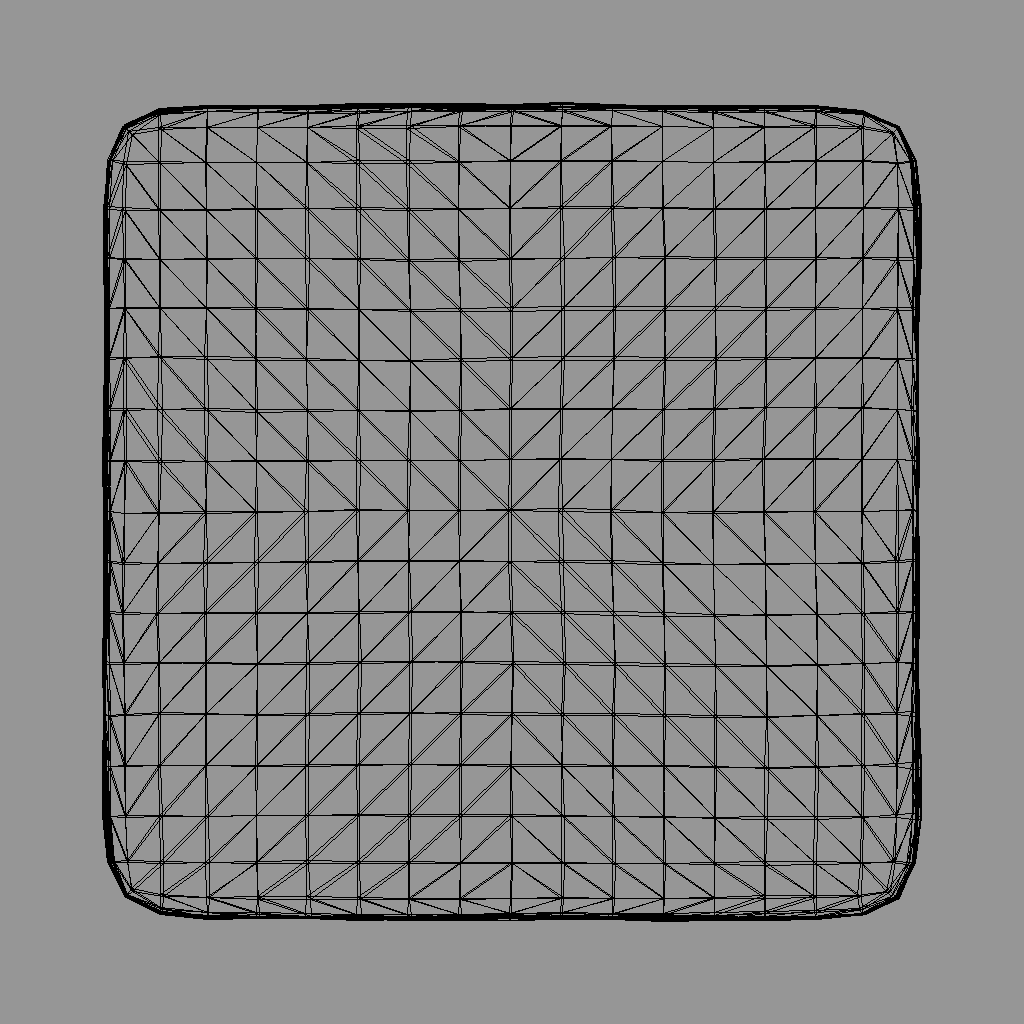
\includegraphics[width=\textwidth]{../output/renders/cube-bruit-0_LissageFacteurDiffusion_5_0.500000.png}
        \caption{Facteur de diffusion ($\alpha=0.5$)}
        \label{fig:res_diffusion}
    \end{subfigure}
    
    \vspace{0.5cm}
    \begin{subfigure}[b]{0.45\textwidth}
        \centering
        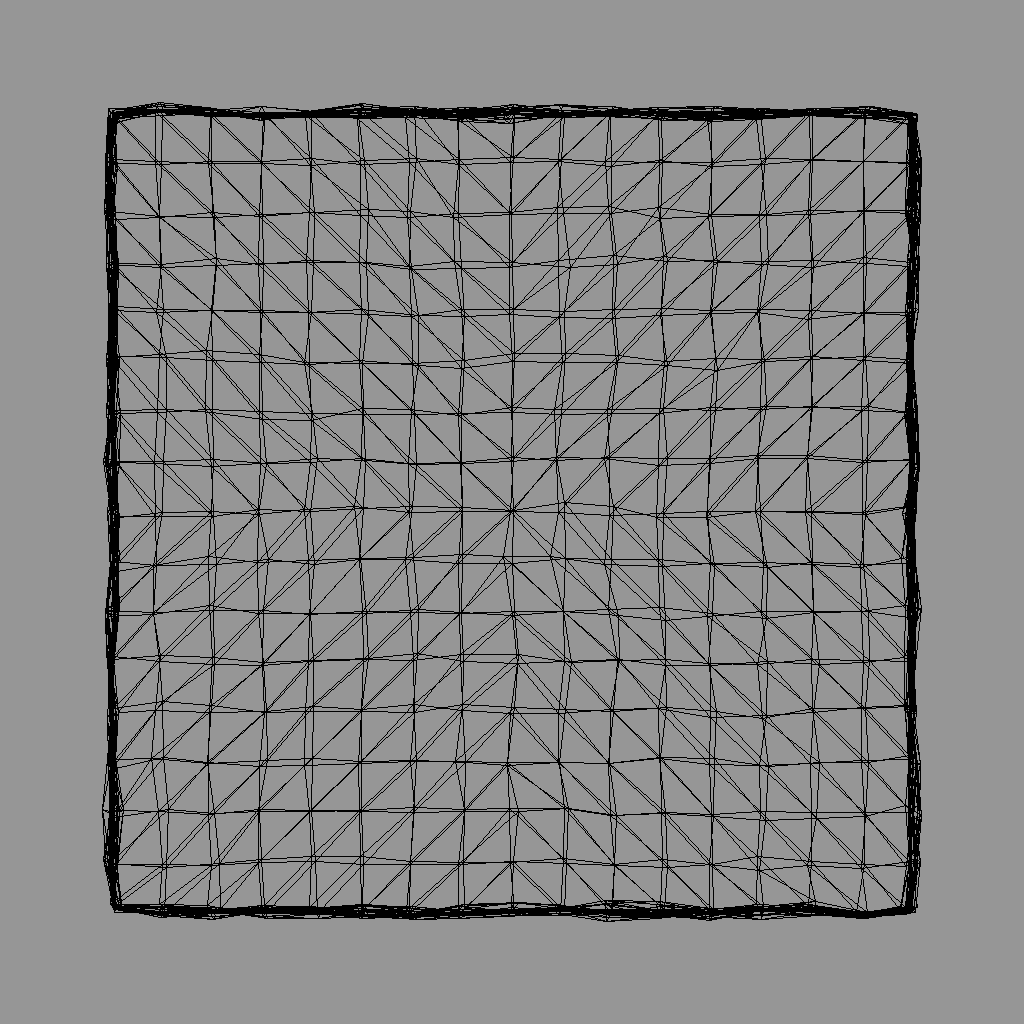
\includegraphics[width=\textwidth]{../output/renders/cube-bruit-0_LissageTaubin_5_0.330000_-0.340000.png} 
        \caption{Taubin ($\lambda=0.33, \mu=-0.34$)}
        \label{fig:res_taubin}
    \end{subfigure}
    \hfill
    \begin{subfigure}[b]{0.45\textwidth}
        \centering
        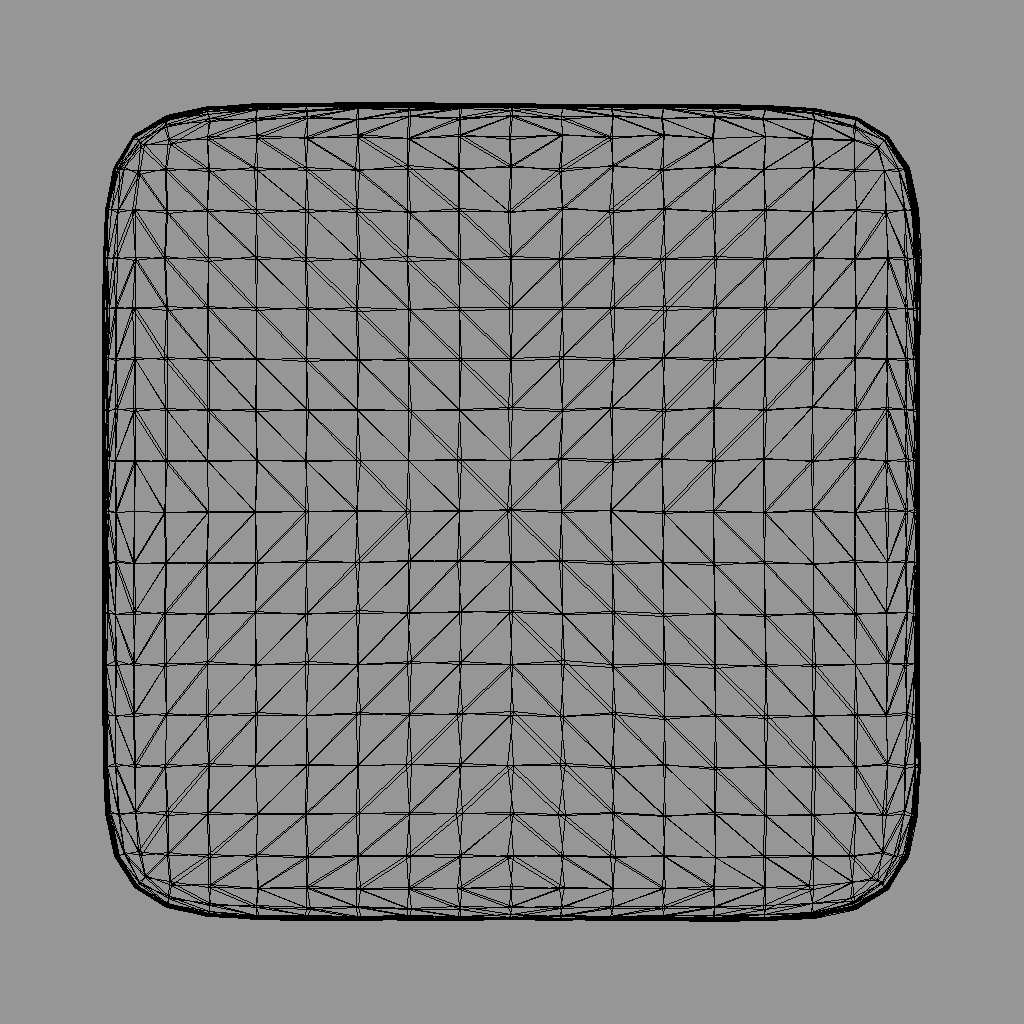
\includegraphics[width=\textwidth]{../output/renders/cube-bruit-0_LissageLaplacienPondere_5_cotangentes.png} 
        \caption{Laplacien Pondéré (Cotangentes)}
        \label{fig:res_cotangent}
    \end{subfigure}
    \caption{Comparaison des résultats de lissage appliqués sur un même maillage bruité (rendu en fil de fer). 5 itérations ont été appliquées pour chaque méthode.}
    \label{fig:comparaison_lissages}
\end{figure}

\subsection{Analyse des performances géométriques}

L'observation des rendus générés met en évidence plusieurs comportements de nos algorithmes qu'il est intéressant de notifier :

\begin{itemize}
    \item \textbf{Lissage Laplacien Uniforme (Fig. \ref{fig:res_laplacien}) :} Comme attendu, les bruits sont gommés. Cependant, on observe un debut phénomène de rétrécissement (\textit{shrinkage}). Les sommets convergent au fur et à mesure vers le centre de masse global de leur voisinage local, écrasant les volumes et adoucissant de manière excessive les arêtes vives du modèle (ici cela s'observe facilement au niveau des coins de notre cube qui se retrouvent rapidement arrondis). 
    \\ L'objet perd ses dimensions initiales et devient au bout de plusieurs itérations assimilable à une boule (voir figure \ref{fig:Laplacien40}).
    \begin{figure}[H]
        \centering
        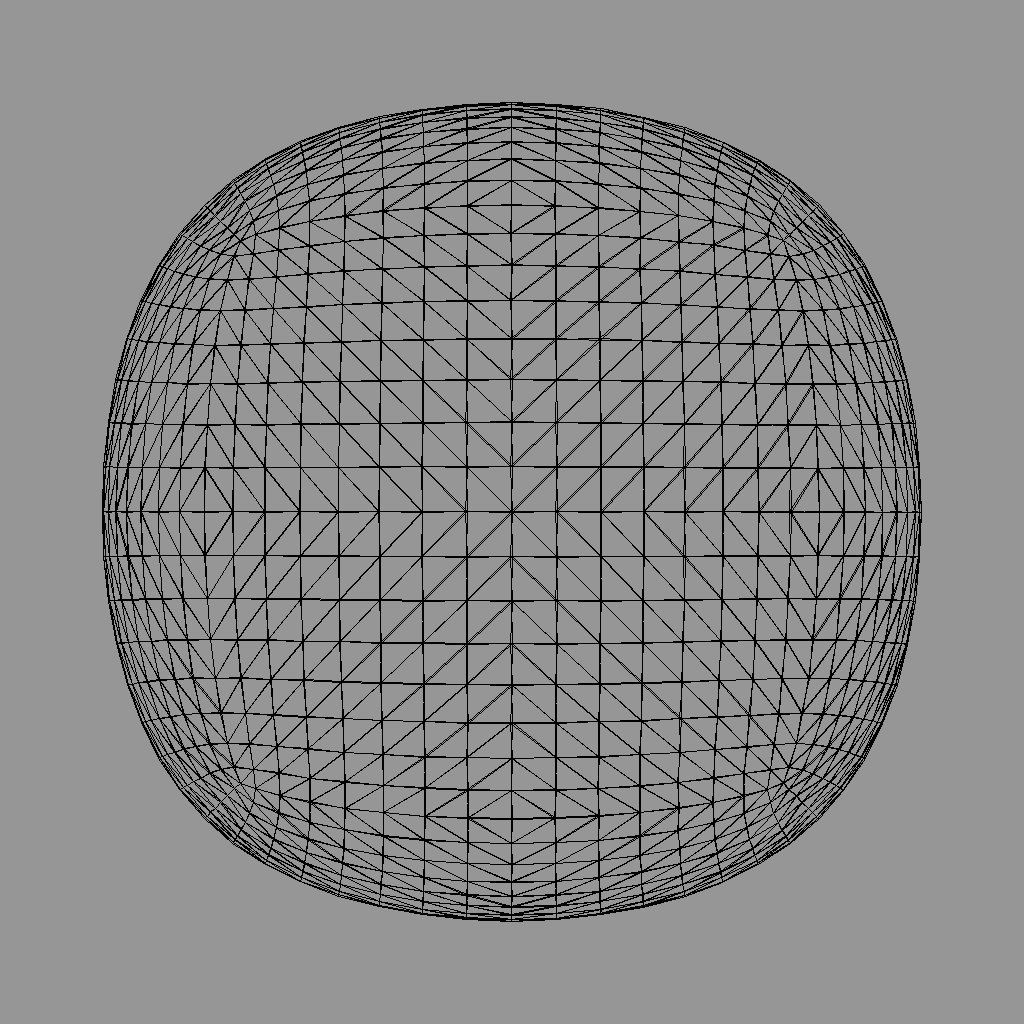
\includegraphics[width=0.40\textwidth]{../output/renders/cube-bruit-0_LissageLaplacien_100.png}
        \caption{Laplacien Uniforme à 100 itérations}
        \label{fig:Laplacien40}
    \end{figure}

    
    \item \textbf{Lissage avec Facteur de Diffusion (Fig. \ref{fig:res_diffusion}) :} L'introduction d'un facteur de pondération $\alpha < 1$ permet de ralentir l'effondrement du volume. 
    Les itérations sont moins agressives et l'état d'équilibre est repoussé, mais le problème topologique de fond persiste.
    
    \item \textbf{Lissage de Taubin (Fig. \ref{fig:res_taubin}) :} Les résultats illustrent parfaitement la robustesse de cette méthode. 
    L'alternance des phases de contraction ($\lambda$) et de dilatation ($\mu$) agit comme un filtre passe-bas très efficace. 
    Cependant, ces successions de contractions et dilatations demandent plus d'itérations afin d'obtenir des résultats visuellement plus qualitatifs. C'est pour cela que sur la figure \ref{fig:res_taubin}, nous ne percevons pas encore les effets du filtrage des bruits.
    En regardant en revanche les résultats obtenus après 40 applications du filtre, on observe une bien meilleure conservation des angles que les méthodes précédentes, ainsi qu'une répartition plus homogène des surfaces sur le mesh (voir figure \ref{fig:Taubin40}).
    
    \begin{figure}[H]
        \centering
        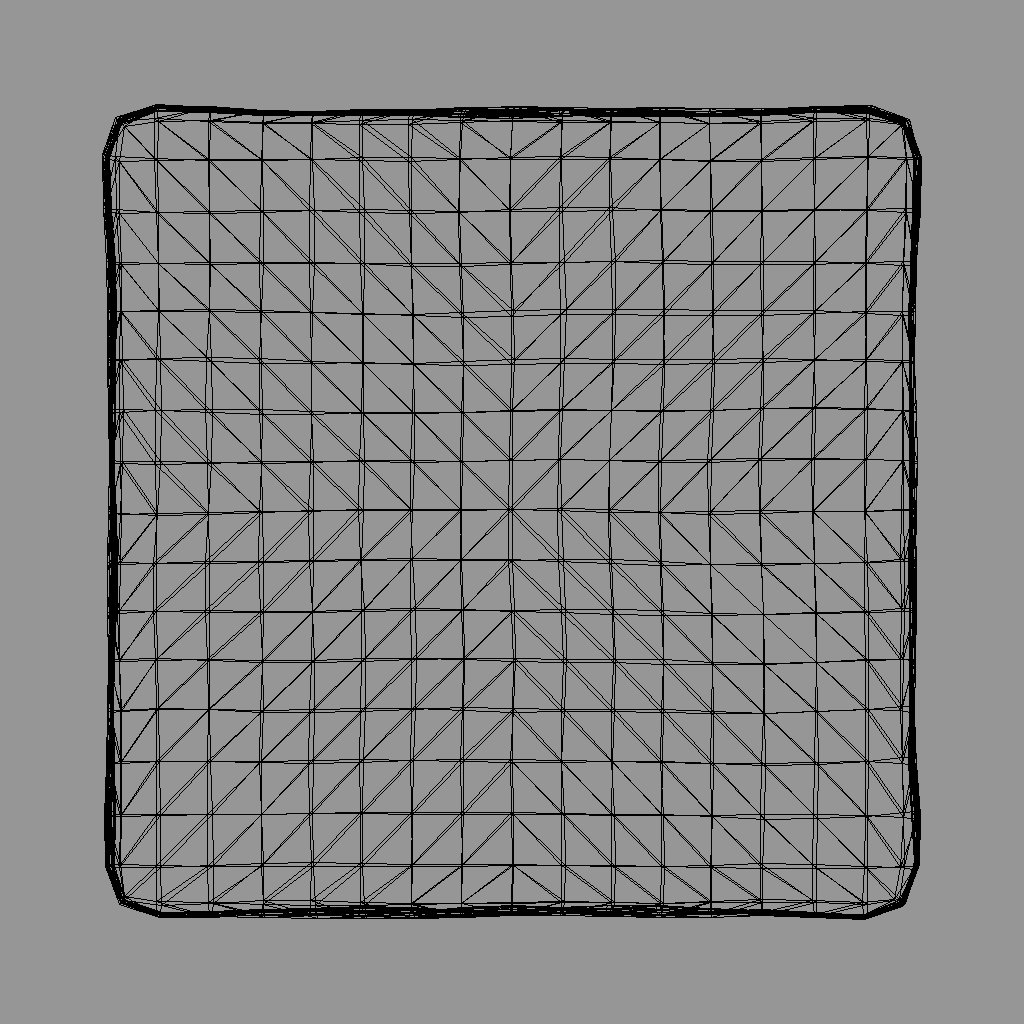
\includegraphics[width=0.40\textwidth]{../output/renders/cube-bruit-0_LissageTaubin_40_0.330000_-0.340000.png}
        \caption{Lissage de Taubin à 100 itérations}
        \label{fig:Taubin40}
    \end{figure}

    
    \item \textbf{Lissage Pondéré par Cotangentes (Fig. \ref{fig:res_cotangent}) :} 
    Cette méthode se démarque en théorie par sa capacité à préserver les singularités géométriques. Cependant, dans le cas particulier d'un cube, les seules courbures
    présentes sont concentrées sur ses arêtes à 90° et ses coins. Ces zones constituent précisément des points de courbure extrême, où les poids cotangents deviennent très grands et exercent une traction disproportionnée sur les
    sommets adjacents, provoquant une érosion des arêtes plutôt que leur préservation.
    Ce comportement est logique avec le calcul même de la cotangente, car cette méthode n'est tout simplement pas adaptée à une géométrie aussi angulaire qu'un cube.
    Sur un maillage présentant une courbure continue et progressive, elle surpasserait théoriquement les autres approches testées.
\end{itemize}

En conclusion, si les méthodes de base (Laplacien simple et diffusion) sont aisées à implémenter, elles se révèlent destructrices pour la géométrie globale. Le choix d'ingénierie se portera préférentiellement sur la méthode de Taubin pour garantir une conservation rigoureuse du volume, ou sur le Laplacien cotangent pour respecter au mieux la géométrie différentielle et les arêtes vives d'une topologie complexe.

\section{Conclusion}

Ce TP nous a permis de développer une compréhension concrète des opérateurs de lissage géométrique en 3D. L'utilisation de CGAL et de ses structures de données en demi-arêtes (\textit{Halfedge Data Structure}) a facilité le parcours topologique des voisinages, étape critique pour l'implémentation d'algorithmes locaux. 

Nous avons pu voir que des approches mathématiquement simples comme le centroïde montrent très vite leurs limites géométriques (rétrécissement, perte de détails). Le passage à des modèles plus robustes, qu'il s'agisse de la compensation de volume par la méthode de Taubin ou de l'approximation de l'opérateur de Laplace-Beltrami par les cotangentes, illustre parfaitement la complexité et la richesse du traitement de la géométrie discrète. Les outils ainsi implémentés forment une base solide pour des processus plus avancés, notamment la segmentation ou la déformation de maillages que nous aborderons par la suite.

    
\end{document}
